\chapter{PSkel-MPPA}
\label{cha:proposta}

Esta seção apresenta as ideias fundamentais que irão embasar a proposta e implementação
da adaptação do \fw \pskel para o processador \mppa.

\section{Visão Geral}

Como dito anteriormente, diversas dificuldades prejudicam o desenvolvimento de aplicações para
processadores \textit{manycore}, tais como o \mppa. Neste projeto, será dado um enfoque para
uma classe de aplicações paralelas que seguem o padrão \stencil. Nesse sentido, adaptar
o \fw PSkel para esse processador trará benefícios claros, simplificando o desenvolvimento
de aplicações \stencil para o \mppa. O \fw fornecerá uma transparência
no particionamento de tarefas e dados para esse ambiente, liberando o desenvolvedor
da utilização de meios de comunicação via \noc. Além disso, aplicações já desenvolvidas para o
\fw poderão ser executadas no \mppa sem a necessidade de nenhuma alteração em
seus códigos originais.

% \todo[inline]{Destacar o que consiste a proposta: 1) que classes serão alteradas? 2) como será feita a comunicação dos dados? 3) será feito uso de técnicas para divisão dos tiles? quais? 4) será dado foco somente para desempenho? ou consumo de energia também? Os resultados obtidos serão comparados com quais outras arquiteturas?}


\begin{figure}[!h]
	\centering
    \caption{Esquemático ilustrando a implementação.}
    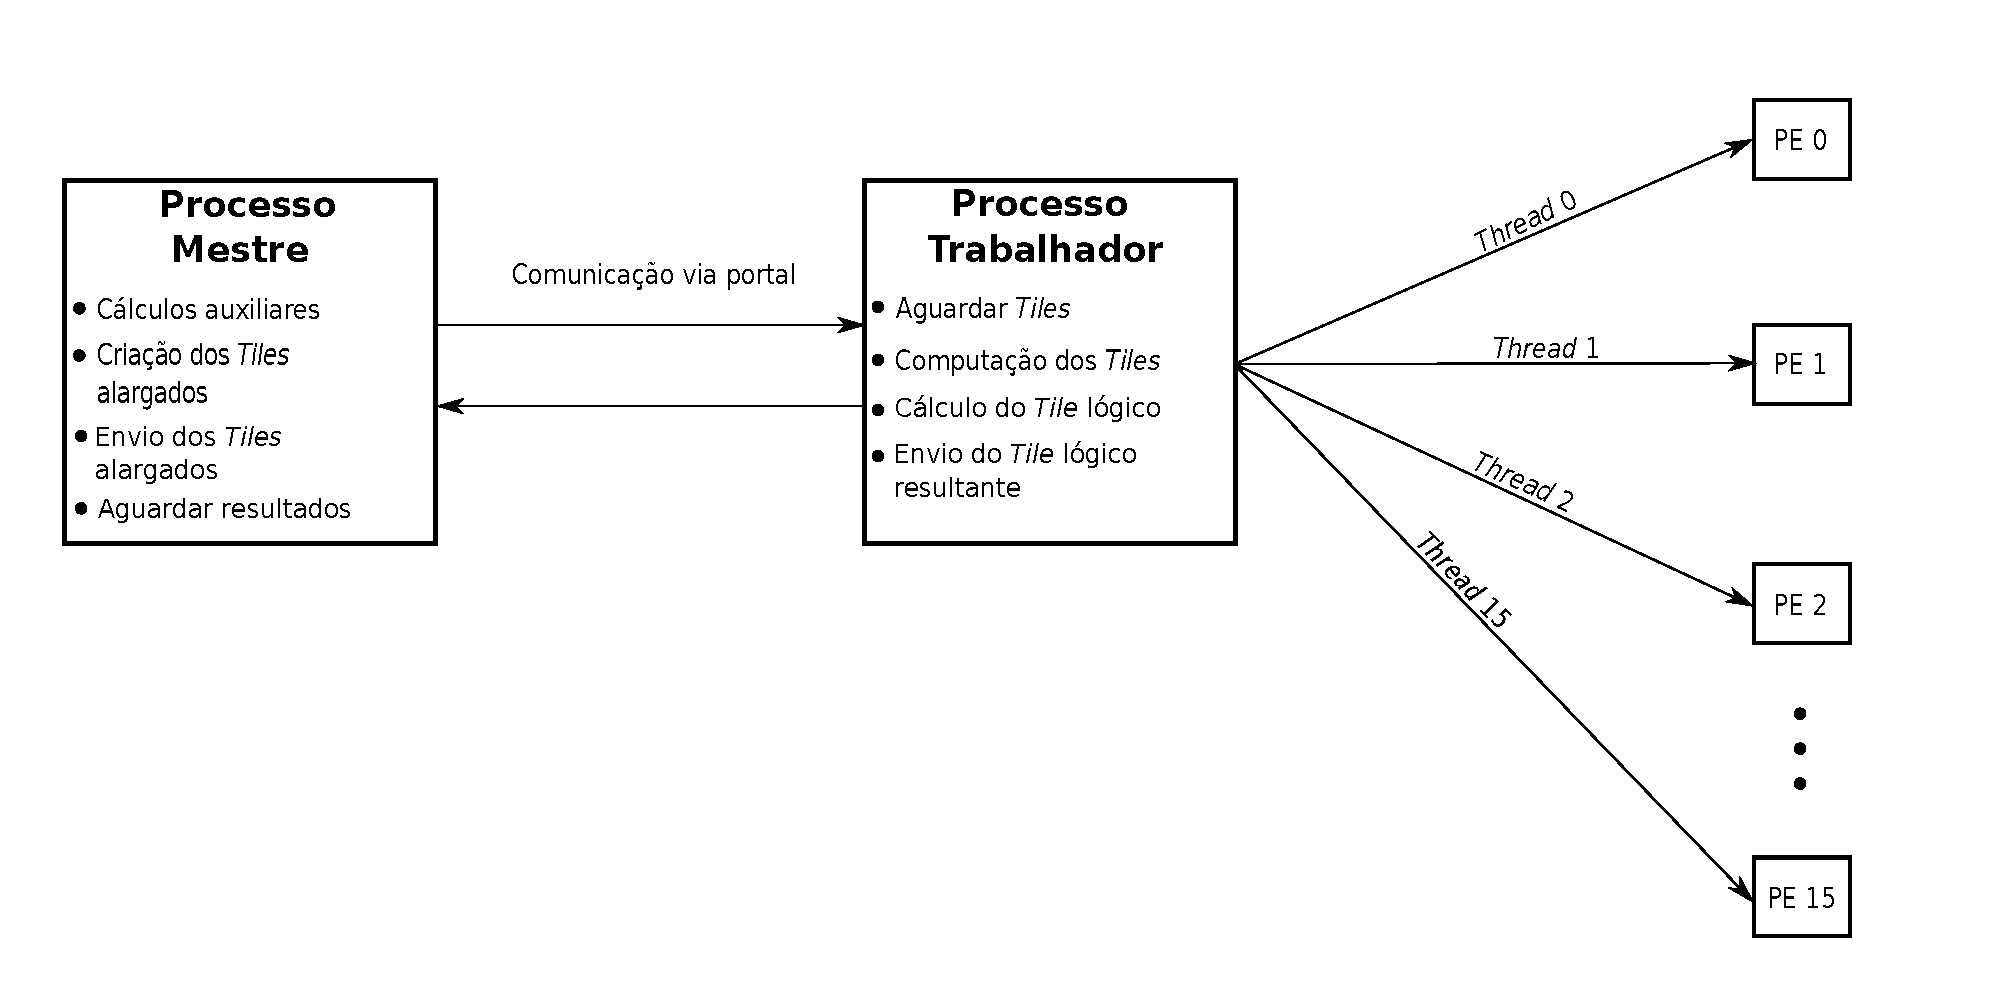
\includegraphics[width=1.2\textwidth, height=7cm]{figs/visaoGeralPSKELMPPA.pdf} \\
    Fonte: Desenvolvido pelo autor.
    \label{fig:visaoGeral}
\end{figure}



A Figura~\ref{fig:visaoGeral} ilustra, de forma simplificada, a adaptação
desenvolvida. A nova adaptação do \fw suporta matrizes \stencil 2D, adotando o modelo
mestre-trabalhador descrito na seção \ref{sec:prog-mppa}. O processo mestre é
executado no subsistema de \es conectado à uma memória LPDDR3, alocando dados de
entrada e saída. Além disso, o processo mestre irá enviar dados para o processo
trabalhador e aguardará os resultados da computação. Por outro lado, o processo
trabalhador é executado em cada \textit{cluster} com o objetivo de realizar a
computação \stencil de forma paralela. A computação será subdividida dentro dos
\textit{clusters} por meio da biblioteca OpenMP, enviando pequenas partes de
dados para cada \pe. Após a computação ser realizada, o resultado é enviado ao
processo mestre. Por fim, toda a comunicação entre os dois processos será
realizada por meio de portais, como especificado na seção \ref{sec:prog-mppa}.

Devido às limitações de memória no \mppa, o mestre deverá enviar para o
trabalhador pequenas partições da matriz de entrada, denominadas de
\textit{tiles}. Durante o processo de subdivisão, cada \textit{tile} deverá
considerar as dependências de vizinhança intrínsecas do padrão \stencil. Mais
precisamente, a computação realizada sobre um elemento de um certo \textit{tile}
poderá possuir uma relação de dependência com outros \textit{tiles} devido à
máscara da computação.


\section{Tiling Trapezoidal}
\label{sec:tiling}
Para tratar os problemas de dependência foi utilizada a técnica de
\textit{tiling} trapezoidal~\cite{meng11} na solução proposta, resultando em redundância de
dados e computações~\cite{rocha17}. Mais especificamente, \textit{tiling} é
geralmente utilizado para particionar a computação de uma aplicação \stencil em
partes menores (\textit{tiles}) entre elementos de processamento\footnote{Nesta
seção, esse termo é utilizado para representar elementos de processamento em
geral, não, necessariamente, os elementos presentes dentro dos \textit{clusters}
no \mppa.}. Essa subdivisão tem como objetivo possibilitar a execução paralela da aplicação.

Contudo, o processo de \textit{tiling} introduz problemas de dependência, pois,
para computar os elementos das bordas de um \textit{tile}, é necessário obter
os valores resultantes em outros elementos de processamento. A Figura~\ref{fig:tilingHalo} ilustra
esse comportamento. As regiões que precisam ser resolvidas por sincronizações e
comunicações entre elementos de processamento é denominada região \textit{halo}. Dependendo do número
de sincronizações e comunicações realizadas, a aplicação pode demorar um tempo
considerável realizando o particionamento de dados entre elementos de
processamento, prejudicando o desempenho da aplicação.

\begin{figure}[!h]
	\centering
    \caption{Esquemático ilustrando a região \textit{halo}.}
    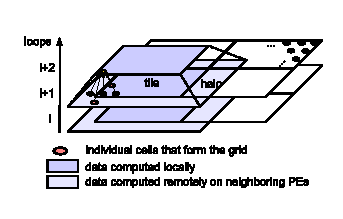
\includegraphics[width=0.6\textwidth]{figs/tilingHalo.pdf} \\
    Fonte:~\cite{meng11}.
    \label{fig:tilingHalo}
\end{figure}



Para contornar essa sobrecarga após cada iteração, um \textit{tile} pode ser
alargado para incluir uma \textit{ghost zone}. A Figura~\ref{fig:tiling} ilustra
essa alternativa, onde a \textit{ghost zone} alarga o \textit{tile}, fazendo-o
sobrepor \textit{tiles} vizinhos por meio de múltiplas regiões \textit{halo}.
Desta forma, elementos de processamento podem gerar mais sobreposições com quantidade proporcional ao
número de iterações da aplicação. Além disso, a mesma figura ilustra o
comportamento da \textit{ghost zone}, onde ela agrupa as iterações em estágios.
Cada estágio realiza operações sobre \textit{tiles} sobrepostos, denominados
trapezóides. Por fim, os trapezóides irão produzir um dado sem sobreposição ao
final da computação de todas as iterações.

\begin{figure}[!h]
	\centering
    \caption{Esquemático ilustrando a \textit{ghost zone}.}
    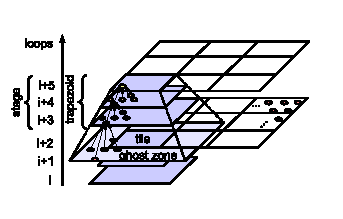
\includegraphics[width=0.6\textwidth]{figs/tiling.pdf} \\
    Fonte:~\cite{meng11}.
    \label{fig:tiling}
\end{figure}



A seguir, a técnica será ilustrada mais profundamente
por meio de definições formais. Seja $A$ uma matriz de dados 2D, com dimensões
$\textrm{dim}(A) = (h,w)$, onde $w$ e $h$ são largura e altura, respectivamente.
Utilizando \textit{tiles} de dimensões ($w'$, $h'$), é possível obter
$\lceil\frac{w}{w^\prime}\rceil\lceil\frac{h}{h^\prime}\rceil$ \textit{tiles}
sobre $A$. Seja $A_{i,j}$ um \textit{tile} seguindo as definições descritas,
onde $0 \leq i < \lceil\frac{w}{w^\prime}\rceil$ e $0\leq j <
\lceil\frac{h}{h^\prime}\rceil$. $A_{i,j}$ possui um \textit{offset} $(i
w^\prime, j h^\prime)$ relativo ao canto superior esquerdo de $A$ e
$\textrm{dim}(A_{i,j}) = (\min\{w^\prime, w-i w^\prime\}, \min\{h^\prime, h-j
h^\prime\})$. O \textit{offset} é um índice de deslocamento necessário para
acessar os elementos de um \textit{tile}.

A Figura~\ref{fig:block2d} ilustra a técnica de \textit{tiling} trapezoidal. Um
\textit{tile} lógico (linha sólida interna) é contido em uma matriz de dados 2D
(linha pontilhada externa) com \textit{offsets} verticais e horizontais dados
por $jh^\prime$ e $iw^\prime$. Se $t$ iterações de uma aplicação \stencil
precisam ser realizadas, é possível computar $t^\prime$ iterações consecutivas
sobre $A_{i,j}$ ($t^\prime \in \left[1,t\right]$) sem a necessidade de nenhuma
troca de dados entre \textit{tiles} adjacentes, isto é, $t^\prime$ iterações
internas. Para realizar iterações consecutivas é necessário utilizar um
\textit{tile} lógico ($A_{i,j}$) alargado com uma \textit{ghost zone} (área
entre a linha sólida interna e a linha sólida externa) que possui uma
\textit{halo region} (área entre a linha sólida interna e a linha pontilhada
interna). Seja $r$ o maior deslocamento necessário sobre a vizinhança de um
elemento, determinado pela máscara \stencil. A área com alcance $r$ que contém a
vizinhança é denominada \textit{halo region}. O número de \textit{halo regions}
que compõem a \textit{ghost zone} é proporcional à $t^\prime$. Desta forma, o
\textit{tile} alargado $A^\ast_{i,j}$ possui um \textit{offset} $(\max\{iw^\prime -
rt^\prime, 0\}, \max\{jh^\prime - rt^\prime, 0\})$ relativo à $A$.

Após a computação das $t^\prime$ iterações consecutivas,
sincronizações devem ser realizadas para resolver as iterações restantes
(iterações externas). Desta forma, $\lceil\frac{t}{t^\prime}\rceil$
sincronizações serão responsáveis por atualizar a matriz de entrada de forma
global.

Devido às dependências de vizinhança presentes na computação \stencil, cada
iteração sobre o \textit{tile} alargado adiciona valores incorretos na
\textit{ghost zone}. A Figura~\ref{fig:errorPropagation} ilustra como que os
valores incorretos se propagam sobre o \textit{tile} alargado. Ao realizar as
iterações, a área útil da \textit{ghost zone} diminui proporcionalmente ao
número de iterações realizadas. Após $t^\prime$ iterações consecutivas, o
\textit{tile} lógico será a região sem erros e sem valores redundantes. Desta
forma, quanto maior for a quantidade de iterações consecutivas, a \textit{ghost
    zone} será maior e, consequentemente, maior a quantidade de computações
redundantes para computar corretamente o \textit{tile} lógico. Portanto, existe
um \textit{trade-off} entre o custo de computação redundante e o número de
comunicações e sincronizações realizadas.
%na \noc durante o processamento de computações
%\stencil iterativas no \mppa.

\begin{figure}[!h]
  \begin{minipage}[b]{0.9\textwidth}
	\centering
    \caption{\textit{tiling} 2D.}
    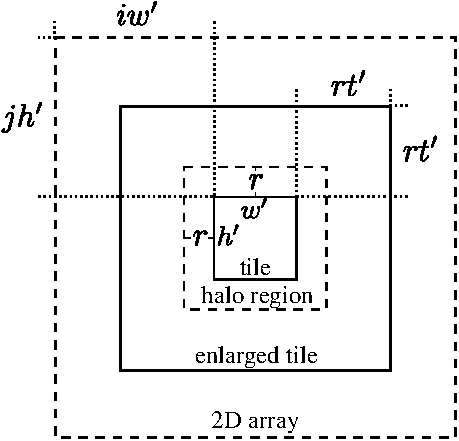
\includegraphics[height=5cm]{figs/tile.pdf} \\
    Fonte:~\cite{rocha17}
	\label{fig:block2d}
  \end{minipage}
\end{figure}

\begin{figure}[!h]
  \begin{minipage}[b]{0.9\textwidth}
	\centering
    \caption{Propagação do erro sobre o \textit{tile} alargado.}
    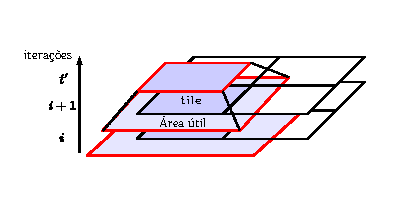
\includegraphics[height=5cm]{figs/tilingProp.pdf} \\
    Fonte: Desenvolvido pelo autor.
    \label{fig:errorPropagation}
  \end{minipage}
\end{figure}

% Na implementação da proposta será necessário modificar classes já existentes
% no \fw para suportar as características do \mppa. Devido à subdivisão da matriz de entrada
% e a comunicação serem diferentes para o \mppa em relação à comunicação
% \cpu-\gpu, classes responsáveis por essas
% operações devem ser modificadas, como, por exemplo, a classe que determina a estrutura
% \textit{Stencil}. Além disso, a comunicação entre os processos mestre e escravo
% do \mppa será feita utilizando portais de comunicação.

% Mais especificamente, uma nova função responsável por subdividir a matriz
% de entrada em pequenas partes (\textit{tiles}), será criada.
% Os \textit{tiles} serão construídos seguindo uma técnica de \textit{tiling}
% trapezoidal~\cite{meng11}, sendo enviados para o processo trabalhador seguindo um modelo de
% escalonamento de tarefas do tipo \textit{round-robin}.
% Para efetuar o envio dos \textit{tiles} será criado um portal de comunicação relacionado com
% cada \textit{tile} da matriz de entrada.
%
% A técnica trapezoidal permite o mestre enviar \textit{tiles} aumentados, isto é,
% \textit{tiles} com uma borda maior, determinada por uma \textit{ghost zone}.
% Desta forma, o processo trabalhador poderá realizar mais de uma iteração sobre
% cada \textit{tile}, diminuindo o número de sincronizações entre os processos.

% A Figura~\ref{fig:tiling} ilustra as modificações sobre o \textit{tile} alargado
% em relação às iterações consecutivas. Mais es

% Devido ao \textit{tile} ser acrescido de uma parte da matriz atribuída a outro
% \textit{tile}, computações redundantes serão realizadas. O tamanho do
% \textit{tile} aumentado pode trazer perda em desempenho em troca de um menor
% número de comunicações entre os processos, isto é, quanto maior o número de
% computações redundantes, menor o número de comunicações. Desta forma, as \textit{ghost zones}
% fornecem uma relação custo-benefício entre computações redundantes e a redução de
% comunicações entre processos.


% Os processos escravos deverão receber os
% \textit{tiles} aumentados enviados pelo mestre, computar o \textit{kernel} da aplicação \stencil
% sobre cada \textit{tile} e enviar o resultado ao mestre.
% Além disso, será possível efetuar iterações sobre o mesmo \textit{tile},
% buscando diminuir o número de comunicações. O \textit{kernel} da aplicação \stencil
% será executado em paralelo em cada \textit{cluster} do \mppa, através do uso da \api OpenMP.
%
% A implementação da proposta será focada em obter ganhos de desempenho e energia
% em relação a outras arquiteturas, como, por exemplo, o processador
% \textit{multicore} Intel Xeon. Desta forma, métodos escolhidos para efetuar a
% comunicação e a subdivisão dos dados serão testados, buscando o melhor método
% para cumprir o foco da proposta.

\section{Implementação}
O processo de execução de uma aplicação no PSkel-MPPA segue a descrição na
seção~\ref{sec:prog-mppa}. A seguir serão apresentadas as funções de cada
processo e como foi realizada a comunicação no \mppa.

\subsection{Processo Mestre}
O processo mestre, executando sobre o subsistema de \es, será responsável por
alocar: os dados de entrada e saída na memória LPDDR3, a máscara da computação e
a estrutura \stencil. O código do processo mestre é idêntico ao código da versão
original do \pskel, contudo o processo mestre não é responsável pela descrição
do \textit{kernel} da computação. O código~\ref{cod:jacobiMestre} mostra a
definição do processo mestre no \mppa.  Na adaptação, a função
\texttt{scheduleMPPA} foi implementada para realizar o controle de dados e a
computação sobre o processador. Ela é encapsulada pela classe
\texttt{Stencil2D}, sendo necessário realizar a passagem de parâmetros definidos
pelo usuário.

\newlength\someheight
\setlength\someheight{3cm}

\begin{figure}[t]
	\begin{lstlisting}[
		caption=Exemplo do código da aplicação Jacobi no processo mestre.,
		label=cod:jacobiMestre,
	]

	int main(int argc, char **argv) {
		/* declaracoes de variaveis omitidas */

		Array2D<float> input(A, M, N);
		Array2D<float> output(B, M, N);
		int neighbors = {{0,1}, {-1,0}, {1,0}, {-1,0}};
		Mask2D<int> mask(4, neighbors);
		struct Arguments args(alpha);

		Stencil2D<Array2D<float>, Mask2D<int>, Arguments>
			jacobi(A, B, args);
		jacobi.scheduleMPPA(slave_bin, threadsNum, clustersNum, tileDim,
                        iterations);

		return(0);
	}
\end{lstlisting}
\end{figure}

Por meio da abstração proveniente do \pskel, o processo mestre irá iniciar a
execução dos processos trabalhadores dentro dos \textit{clusters} no \mppa. A
quantidade de \textit{clusters} utilizados na aplicação é determinada
dinâmicamente em relação à quantidade de \textit{tiles} lógicos e o número de
\textit{clusters} definidos pelo usuário.  Mais precisamente, dado uma entrada
$s$ e um tamanho de \textit{tile} lógico $s^\prime$, a quantidade de
\textit{tiles} lógicos é determinada por $\lceil\frac{s}{s^\prime}\rceil$. Caso
a quantidade de \textit{clusters} definida pelo usuário seja maior que o
resultado da relação apresentada, não é necessário iniciar a execução de todos
os \textit{clusters} definidos. Desta forma, apenas a quantidade de
\textit{clusters} necessária será inciada. Caso contrário, a quantidade
determinada pelo usuário será utilizada.

Em seguida, o processo mestre irá utilizar a técnica de \textit{tiling}
trapezoidal para subdividir a matriz de entrada em \textit{tiles} alargados, e
enviar-los para cada \textit{cluster} seguindo um escalonamento circular
(\textit{round-robin}).  Devido a isso, alguns \textit{clusters} podem receber
mais \textit{tiles} que outros, dependendo do número de \textit{tiles} e
\textit{clusters} utilizados na computação. Ao finalizar a subdivisão dos dados,
o processo mestre irá enviar os \textit{tiles} alargados para o processo
trabalhador. Para efetuar a subdivisão por meio da técnica de \textit{tiling}
trapezoidal são necessários cálculos para determinar variáveis que são
modificadas dinâmicamente, como, por exemplo, endereços de memória da
\textit{ghost zone} e a posição do \textit{tile} lógico na matriz de entrada.
Mais precisamente, esses cálculos serão realizados para fornecer os
\textit{offsets} necessários para a função \texttt{tiling} da classe
\texttt{StencilTiling}. Essa função é responsável por retornar os endereços de
memória corretos de cada \textit{tile} alargado. Desta forma, para determinar
precisamente os endereços de memória de cada \textit{tile} alargado são
necessários alguns fatores: i) parâmetros definidos pelo usuário, como o tamanho
dos dados de entrada, tamanho dos \textit{tiles} lógicos e o número de
iterações; ii) parâmetros do \stencil \textit{kernel}, como o tamanho da
máscara. iii) os \textit{offsets} do \textit{tile} lógico em relação à matriz de
entrada. Por fim, processo mestre espera os \textit{clusters} finalizarem a
execução e agrupará os \textit{tiles} resultantes em um único \texttt{Array2D}
de saída. Caso existam mais iterações, será necessário armazenar os resultados
enviados pelos \textit{clusters} em uma matriz auxiliar, permitindo a realização
de sincroninzações entre o processo mestre e trabalhador.

Mais precisamente, os processos trabalhadores irão realizar iterações internas
($t^\prime$), enquanto o processo mestre irá realizar iterações externas
($\lceil\frac{t}{t^\prime}\rceil$). Após a computação de todas as iterações
internas pelos processos trabalhadores, será necessário uma sincronização entre
o processo mestre e os processos trabalhadores. Essa sincronização permitirá que
o processo mestre atualize uma matriz auxiliar com resultados temporários,
utilizando-a como base para os novos envios de \textit{tiles} alargados em uma
nova iteração externa. Com isso, é possível remover valores incorretos
calculados dentro da \textit{ghost zone} e atualizar os dados para todos os
\textit{clusters}, eliminando problemas de dependência.

A comunicação entre o processo mestre e o processo trabalhador é realizada por
meio de portais de comunicação inicializados em cada processo. A
seção~\ref{sec:comunicacao} descreve mais profudamente as características da
comunicação na implementação.

A Figura~\ref{fig:visaoGeralMestre} ilustra o esquemático atualizado da visão geral
da proposta considerando as características do processo mestre.


\begin{figure}[!h]
	\centering
    \caption{Esquemático ilustrando a implementação mais aprofundada do processo mestre.}
    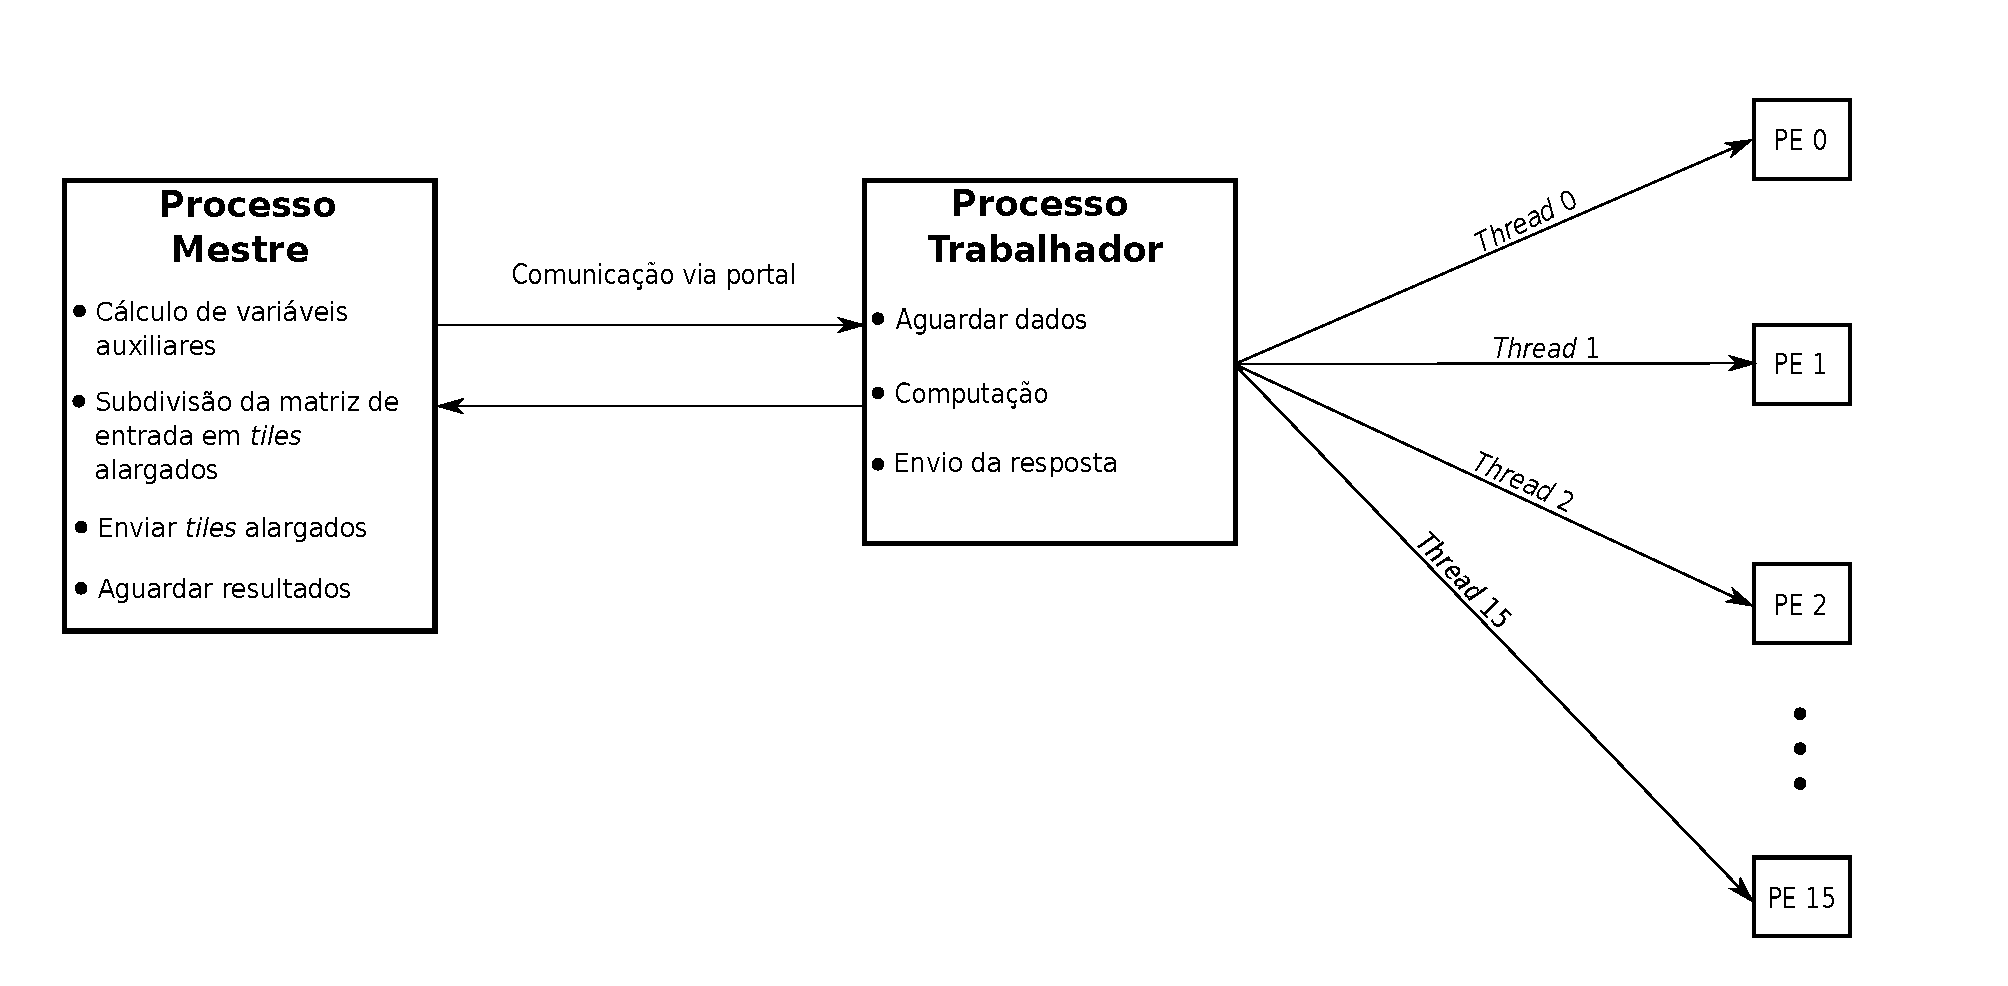
\includegraphics[width=1.2\textwidth, height=7cm]{figs/visaoGeralPSKELMPPAMestre.pdf} \\
    Fonte: Desenvolvido pelo autor.
    \label{fig:visaoGeralMestre}
\end{figure}



\subsection{Processo Trabalhador}
Os processos trabalhadores serão responsáveis pela
execução do \textit{kernel} da computação. Essa fase pode ser dividida em
etapas: i) Cada processo trabalhador irá receber o \textit{tile} alargado.
ii) iterações internas são computadas sobre o \textit{tile} alargado. iii)
cálculo de \textit{offsets} para determinar o espaço de endereçamento do
\textit{tile} lógico e enviá-lo ao processo mestre. Após cada \textit{tile}
alargado atribuído ao processo trabalhador ser computado, todos os processos
trabalhadores precisam sincronizar em uma barreira. Para cumprir esse objetivo,
são utilizadas funções de baixo nível do \mppa. A sincronização é realizada
junto com o mestre, com o objetivo de atualizar a matriz auxiliar para uma nova
sequência de envios de \textit{tiles}. Esse processo é repetido até
todas as sincronizações (iterações externas) serem realizadas.

Mais precisamente, o processo trabalhador irá receber o \textit{tile}
alargado, atribuído pelo processo mestre, por meio de portais de comunicação.
A computação será efetuada sobre os dados recebidos com o auxílio da biblioteca
OpenMP. Desta forma, será possível distribuir a computação entre os \pes dentro
do \textit{cluster}. Será realizada a computação do \textit{tile} alargado por
$t^\prime$ iterações internas. Após todas as iterações serem realizadas, o
processo trabalhador terá que efetuar cálculos, com \textit{offsets} enviados
pelo processo mestre, para determinar o endereço de memória do \textit{tile}
lógico dentro do \textit{tile} alargado. Essa ação deve ser realizada para
filtar os valores incorretos provenientes da computação do \textit{tile}
alargado. Por fim, o \textit{cluster} irá enviar o \textit{tile} lógico para o
processo mestre. Ao completar o envio, os processos trabalhadores terão que
sincronizar com o processo mestre e outros processos trabalhadores por meio de
uma barreira, caracterizando uma iteração externa. Mais detalhes sobre a
comunicação do processo trabalhador com o processo mestre serão abordados na
seção~\ref{sec:comunicacao}.

%  Como descrito na seção~\ref{}, a técnica de
% \textit{tiling} trapezoidal auxilia a execução de iterações sobre um único
% \textit{tile}, fornecendo um menor número de comunicações entre processos mestre
% e trabalhador aumentando a carga da computação. Esse aumento de carga é devido a
% região \textit{halo} que é acrescida ao \textit{tile} lógico. Desta forma,
% devido à característica da computação \stencil

% As ações descritas serão efetuadas para todos os \textit{tiles} alargados
% atribuídos ao processo trabalhador. Além disso, ao finalizar o envio dos
% \textit{tiles} resultantes, o processo trabalhador terá que efetuar uma
% sincronização junto ao processo mestre.
%
O código~\ref{cod:jacobiTrabalhador} mostra a definição do processo trabalhador
no \mppa. Este processo será responsável por descrever o \textit{kernel} da
computação e, também, estruturas de dados de forma similar ao processo mestre.
Devido aos valores de \textit{offsets} e variáveis importantes para a computação
do \textit{kernel} serem geradas dinâmicamente, o processo trabalhador precisa
receber do processo mestre, além do \textit{tile} alargado, variáveis
responsáveis por controlar a comunicação. Dentre elas, temos variáveis indicando
as dimensões do \textit{tile} a ser recebido, número de iterações totais e
\textit{offsets} para auxiliar a comunicação. Por fim, as ações de recebimento,
computação e envio de \textit{tiles} foram encapsuladas pela função
\texttt{runMPPA}, tornando todas as fases descritas para o processo
trabalhador transparentes ao usuário.


\begin{figure}[!h]
    \begin{lstlisting}[
		caption=Exemplo do código da aplicação Jacobi no processo trabalhador.,
		label=cod:jacobiTrabalhador,
	]
	__parallel__ void
	stencilKernel(Array2D<float> A, Array2D<float> B, Mask2D<int> mask,
								struct Arguments args, int x, int y){
		B(x,y) = args.alpha * (A(x,y+1) + A(x,y-1) + A(x+1,y)
                           + A(x-1,y));
	}

	int main(int argc, char **argv) {
		/* declaracoes de variaveis omitidas */

		Array2D<float> inputTile(A, M, N);
		Array2D<float> outputTile(B, M, N);
		int neighbors = {{0,1}, {-1,0}, {1,0}, {-1,0}};
		Mask2D<int> mask(4, neighbors);
		struct Arguments args(alpha);

		Stencil2D<Array2D<float>, Mask2D<int>, Arguments>
			jacobi(A, B, mask, args);
		jacobi.runMPPA(cluster_id, numThreads, numTiles, iterations);

		return(0);
	}
\end{lstlisting}
\end{figure}

A Figura~\ref{fig:visaoGeralTrabalhador} ilustra a visão geral da implementação
atualizada com as características do processo trabalhador.

\begin{figure}[!h]
	\centering
    \caption{Esquemático ilustrando a implementação mais aprofundada do processo trabalhador.}
    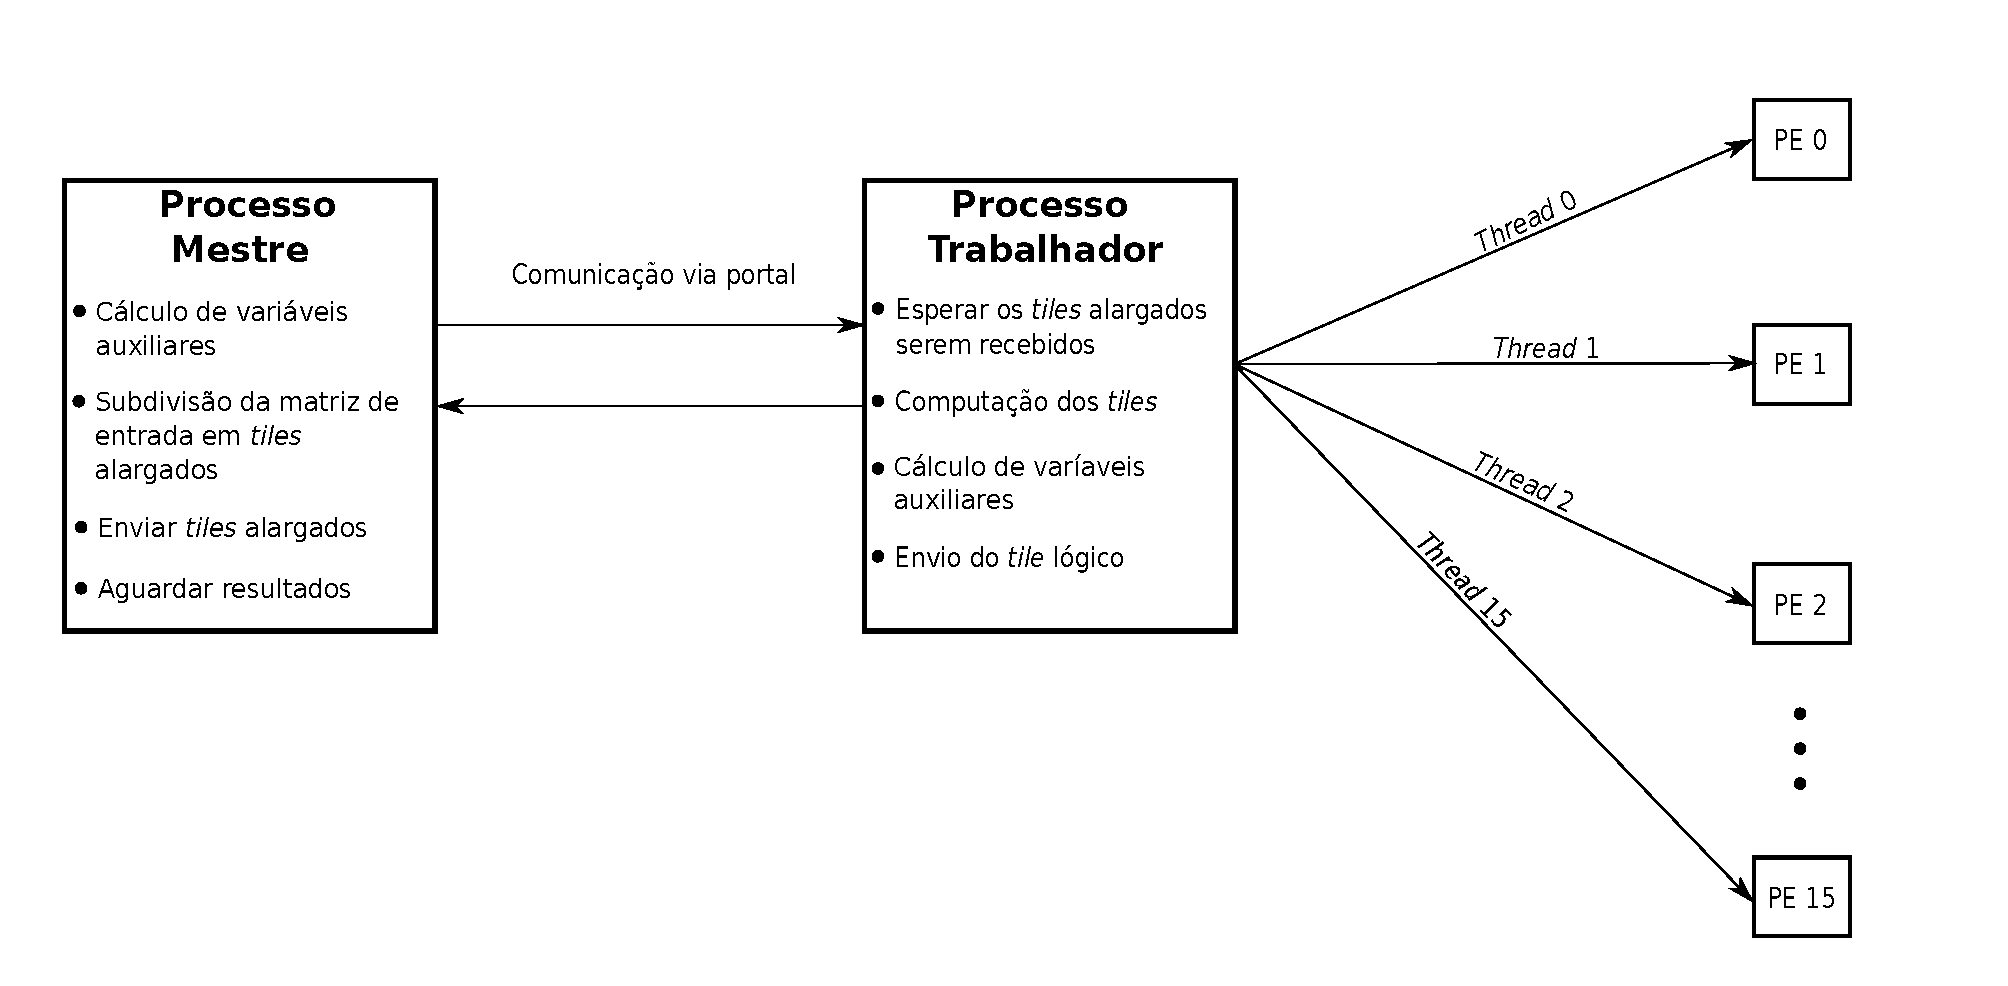
\includegraphics[width=1.2\textwidth, height=7cm]{figs/visaoGeralPSKELMPPATrabalhador.pdf} \\
    Fonte: Desenvolvido pelo autor.
    \label{fig:visaoGeralTrabalhador}
\end{figure}


\subsection{Comunicação}
\label{sec:comunicacao}

Para efetuar a comunicação, o processo mestre cria portais de escrita e leitura
por meio de funções de baixo nível do \mppa. A criação dos portais são encapsulados pela
estrutura \texttt{Array2D}. Desta forma, ao ser criado um \texttt{Array2D},
portais de escrita e leitura podem ser vinculados à ele. Por sua vez, o
processo trabalhador irá criar estruturas \texttt{Array2D} temporárias para
receber o \textit{tile} alargado.

Devido as operações sobre \textit{tiles} e matrizes serem realizadas sobre
endereços de memória, quando o processo mestre ou trabalhador deseja enviar um
dado, é necessário que ele se apresente contíguo na memória. Caso contrário,
dados incorretos podem ser enviados devido à posição deles na memória. Mais
precisamente, essa é uma restrição da \api e da \noc no \mppa, onde os dados
armazenados em cada \textit{tile} precisam ser contíguos para serem transferidos
pela \noc. Uma solução com cópias locais de dados é simples e contorna o
problema, contudo o tempo para efetuar a cópia de um \textit{tile} cresce
proporcionalmente com o seu tamanho e desperdiça memória. Desta forma, com o
objetivo de evitar cópias locais de dados, utiliza-se o conceito de
\textit{strides}. Cada stride é uma parte contígua do \texttt{Array} original,
sendo determinado por deslocamentos (\textit{offsets}) especificados durante a
execução. Os \textit{offsets} são dinâmicos e dependem dos \textit{tiles} sendo
computados. Essas informações são conhecidas pelo processo mestre
por meio da utilização da classe \texttt{StencilTiling}. Por outro lado, o
processo trabalhador recebe essas informações do processo mestre.

A Figura~\ref{fig:strides} ilustra o processo de comunicação com o método
\textit{strides}. Mais precisamente, ao determinar o endereço inicial do
\textit{tile}, pode-se definir "saltos"{} que podem ser realizados sobre a
memória local (\textit{source}). Utilizando como exemplo a figura~\ref{fig:strides}, o endereço inicial
do \textit{tile} está em $init+(4 * size)$, onde $size$ é o tamanho, em bytes,
do tipo armazenado pela matriz e $init$ é o endereço incial da matriz. O tamanho
do "salto"{} realizado pelo método é determinado pela largura da matriz de
entrada, enquanto a quantidade de "saltos"{} é determinada pela altura do
\textit{tile}. Além disso, a quantidade de dados após o endereço inicial do
\textit{tile} precisa ser determinada (\ie área útil), onde, no exemplo, o
\textit{tile} possui $4$ elementos de área útil. O tamanho dos "saltos"{} é
relativo ao endereço inicial do \textit{tile}, então, esse parâmetro deve
contabilizar, também, a área útil do \textit{tile}. Ao realizar todos os
"saltos"{}, o método irá enviar diretamente, via portal, os dados especificados
pelo endereço incial do \textit{tile} e pelos "saltos"{} na memória com a área útil
especificada. Com isso, é possível enviar de forma contígua e direta os
\textit{tiles} à outro processo, sem a necessidade de cópias locais.

\begin{figure}[!h]
	\centering
    \caption{Exemplo do funcionamento do método \textit{strides} no \mppa.}
	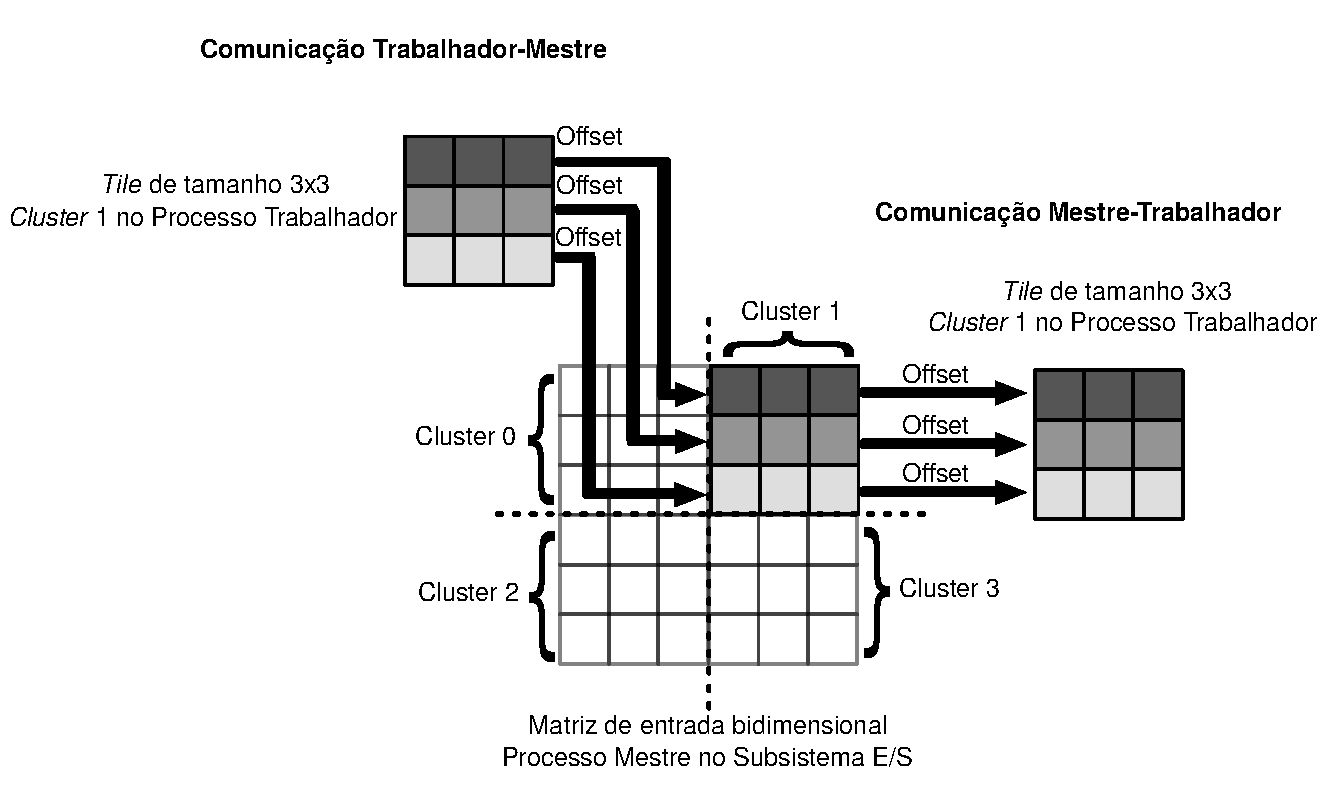
\includegraphics[width=0.9\textwidth]{figs/stridesImage.pdf} \\
    Fonte: Desenvolvido pelo autor.
	\label{fig:strides}
\end{figure}

Por outro lado, o processo trabalhador precisa enviar apenas o \textit{tile}
lógico. Desta forma, o endereço inicial para envio não será modificado, contudo
é necessário especificar a quantidade e tamanho dos "saltos"{}. A quantidade de
"saltos"{} é determinada pela altura do \textit{tile}, enquanto o tamanho dos
"saltos"{} e a área útil é igual à largura do \textit{tile}. Com o método
\textit{strides} é possíveli, também, determinar "saltos"{} no endereço de
memória do processo destino (\textit{target}). O processo trabalhador precisa
enviar o \textit{tile} resultante na posição de memória correta no processo
mestre.  Portanto, ele irá utilizar um deslocamento $(heightOffset * width) +
widthOffset$ sobre o \textit{target}, onde $heightOffset$ é o deslocamento
relativo à altura, $width$ é a largura do \textit{tile} e $widthOffset$ é o
deslocamento relativo à largura. No exemplo adotado, essas variáveis são,
respectivamente, $0$, $4$ e $4$. O processo mestre não utiliza essa função do
método, pois não é necessário inserir o \textit{tile} em uma posição de memória
específica no processo trabalhador.

Por fim, para fornecer uma maior facilidade ao usuário, a técnica de
\textit{tiling} utilizada, as comunicações via \noc e adaptações foram
realizadas dentro do \textit{back-end} do \pskel.
